\documentclass[10pt,twoside]{article}
\usepackage[utf8]{inputenc}
\usepackage{amsmath}
\usepackage{amsfonts}
\usepackage{amssymb}
\usepackage[spanish,es-noshorthands]{babel}
\usepackage[T1]{fontenc}
\usepackage{lmodern}
\usepackage{graphicx,hyperref}
\usepackage{tikz,pgf}
\usepackage{multicol}
\usepackage{subfig}
\usepackage[papersize={6.5in,8.5in},width=5.5in,height=7in]{geometry}
\usepackage{fancyhdr}
\pagestyle{fancy}
\fancyhead[LE]{\url{www.autistici.org/mathgerman}}
\fancyhead[RE]{}
\fancyhead[RO]{matematicas.german@gmail.com}
\fancyhead[LO]{}

\author{Germ\'an Avenda\~no Ram\'irez~\thanks{Lic. Mat. U.D., M.Sc. U.N.}}
\title{\begin{minipage}{.2\textwidth}

\includegraphics[height=1.75cm]{Images/logo-colegio.png}\end{minipage}
\begin{minipage}{.55\textwidth}
\begin{center}
Taller Funciones \\
Cálculo $11^{\circ}$
\end{center}
\end{minipage}\hfill
\begin{minipage}{.2\textwidth}

\includegraphics[height=1.75cm]{Images/logo-sed.png} 
\end{minipage}}
\date{}
\begin{document}
\maketitle
\begin{minipage}{.95\textwidth}
\fbox{\textit{No raye ni dañe esta copia, para que pueda ser utilizada por otro compañero}}
\end{minipage}
\section{Gráficas de funciones}
Si una función $ f $ tiene dominio $ A $, entonces la gráfica de $ f $ es el conjunto de las parejas ordenadas
\[ \{(x,f(x)) | x \in A\} \]
Es decir, la gráfica de $ f $ es el conjunto de todos los puntos $ (x,y) $ tal que $ y=f(x) $; esto es, la gráfica de $ f $ es la gráfica de la ecuación $ y=f(x) $\\

Las gráficas de las funciones se pueden predecir de alguna manera, teniendo en cuenta las siguientes pautas:
\subsection{Función constante}
Toda función de la forma $ f(x)=c $, donde $ c $ es una constante, tiene como gráfica una recta horizontal. Por ejemplo la función $ f(x)=3 $, es una recta horizontal, ya que la imagen todo número real $ x $ es 3.
\subsection{Rectas}
Toda función de la forma $ f(x)=mx+b $, es una recta, donde $ m $ es la pendiente de la recta y $ b $ determina el punto de corte con el eje $ y $.
\subsubsection{Ejemplo:} 
\begin{minipage}{0.45\textwidth}
Grafique la función $ y=-3x+2 $. En este caso, el punto de corte con el eje $ y $ es 2 y tiene pendiente negativa $ -3 $, lo cual indica que la recta es descendente. La gráfica se puede obtener facilmente haciendo una pequeña tabla así:\\

\begin{tabular}{|c|c|}\hline
$x$&$ f(x) $\\ \hline
$ -2 $ & 8\\ \hline
$ 0 $ & 2\\ \hline
2 & $ -4 $\\\hline
\end{tabular}
\vspace{12pt}

Con estos tres puntos es suficiente para hacer la gráfica, la cual queda así:
\end{minipage}\hfill
\begin{minipage}{0.45\textwidth}
  \begin{tikzpicture}[scale=0.45]
\draw[<->] (-3,0) -- (3,0) node[right] {$x$};
\draw[<->] (0,-5) -- (0,9) node[left] {$ y $};
\draw[smooth,domain=-2:2]
plot (\x,-3*\x+2);
\filldraw (0,2) circle (1.5pt)
(2,-4) circle (1.5pt)
(-2,8) circle (1pt);
\node[right]at (0.5,1) {$ y=-3x+2 $};
\node[left] at (-2,8) {$ (-2,8) $};
\node[left] at (0,2) {$ (0,2) $};
\node[left] at (2,-4) {$ (2,-4) $};
\end{tikzpicture}
\end{minipage}
\subsection{Graficando otras funciones}
\begin{minipage}{0.45\textwidth}
En clases anteriores ya hemos hecho las gráficas de las funciones $ y=x^2 $ y $ y=\sqrt{x} $. Ahora observaremos la gráfica de la función $ g(x)=x^3 $. Para hacer su gráfica, primero haremos una tabla así:\\

  \begin{tabular}{|c|c|}\hline
$x$ & $ g(x)=x^3 $\\\hline 
$ -2 $ & $ -8 $\\\hline
$ -1 $ & $ -1 $ \\ \hline
$ -\frac{1}{2} $ & $ -\frac{1}{8} $\\\hline
$ 0 $ & $ 0 $\\\hline
$ \frac{1}{2} $ & $ \frac{1}{8} $\\\hline
1 & 1\\\hline
2 & 8 \\\hline
\end{tabular}
\end{minipage}\hfill
\begin{minipage}{0.45\textwidth}
  \begin{tikzpicture}[scale=0.45]
  \draw[<->] (-3,0)--(3,0) node[right] {$ x $}; 
  \draw[<->] (0,-9)--(0,9) node[left] {$ y $};
  \draw[smooth,domain=-2:2] plot (\x,\x^3) node[right]{$ g(x)=x^3 $}; 
  \filldraw (-2,-8) circle (1pt) node[left] {$ (-2,-8) $}; 
  \end{tikzpicture}
\end{minipage}

\section{TALLER}
\begin{enumerate}
  \item Haga una tabla de valores para hacer la gráfica de las siguientes funciones
  \begin{multicols}{2}
    \begin{enumerate}
      \item $ f(x)=2 $ \item $ f(x)=2x-4 $
      \item $ f(x)=-3 $ \item $ f(x)=6-3x $
      \item $ f(x)=-x+3 \qquad -3\leq x\leq 3$ \item $ f(x)=\dfrac{x-3}{2}, \qquad 0\leq x\leq5 $
      \item $ f(x)=-x^2 $ \item $ f(x)=x^2-4 $
      \item $ g(x)=x^3-8 $ \item $ g(x)=4x^2-x^4 $
      \item $ g(x)=\sqrt{x+4} $ \item $ g(x)=\sqrt{-x} $
      \item $ F(x)=\dfrac{1}{x} $ \item $ F(x)=\dfrac{1}{x+4} $
      \item $ H(x)=|2x| $ \item $ H(x)=|x+1| $
      \item $ G(x)=|x|+x $ \item $ G(x)=|x|-x $
      \item $ f(x)=|2x-2| $ \item $ f(x)=\dfrac{x}{|x|} $
      \item $ g(x)=\dfrac{2}{x^2} $ \item $ g(x)=\dfrac{|x|}{x^2} $
    \end{enumerate}
  \end{multicols}
  \begin{minipage}{0.55\textwidth}
  \item Dada la gráfica de la función $ h $
  \begin{enumerate}
    \item Encuentre $ h(-2),\; h(0),\;h(2), $ y $ h(3) $
    \item Encuentre el dominio y el rango de $ h $
  \end{enumerate}    
  \end{minipage}\hfill
\begin{minipage}{.4\textwidth}
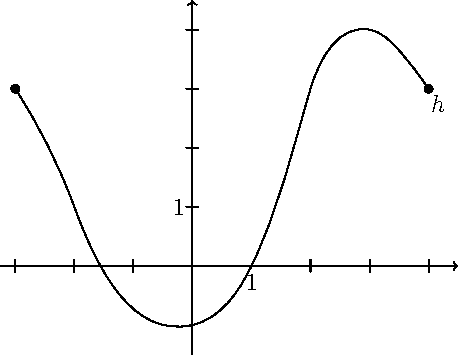
\includegraphics[scale=.75]{asys/funcion_h.pdf} 
\end{minipage}
\begin{minipage}{.4\textwidth}
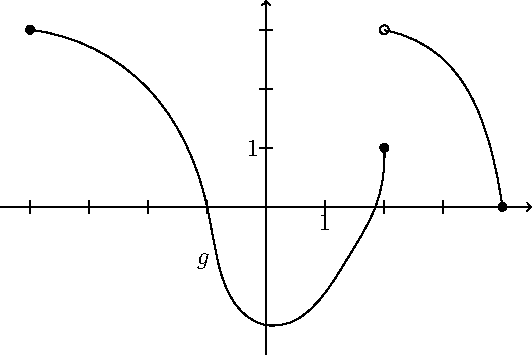
\includegraphics[scale=.75]{asys/funcion_g.pdf} 
\end{minipage}\hfill
\begin{minipage}{.5\textwidth}
  \item Dada la gráfica de la función $ g $
  \begin{enumerate}
    \item Encuentre $ g(-4), g(-2), g(0), g(2) $ y $ g(4) $
    \item Encuentre el dominio y rango de $ g $
  \end{enumerate}
\end{minipage}
\begin{minipage}{.55\textwidth}
  \item Dadas las gráficas de las funciones $ f $ y $ g $
  \begin{enumerate}
    \item ¿Cuál es mayor, $ f(0) $ o $ g(0) $?
    \item ¿Cuál es mayor, $ f(-3) $ o $ g(-3) $?
    \item ¿Para cuáles valores de $ x $, es $ f(x)=g(x) $?
  \end{enumerate}
\end{minipage}\hfill
\begin{minipage}{.4\textwidth}
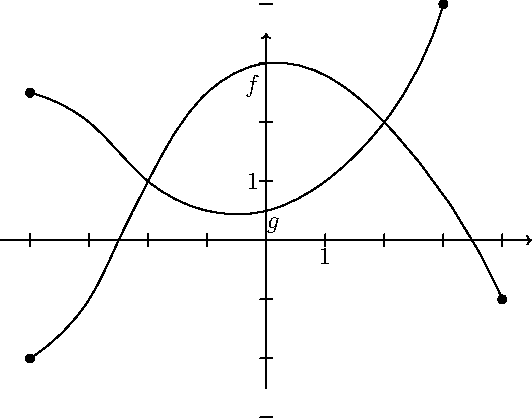
\includegraphics[scale=.6]{asys/funciones_f_g.pdf} 
\end{minipage}
  \begin{minipage}{.45\textwidth}
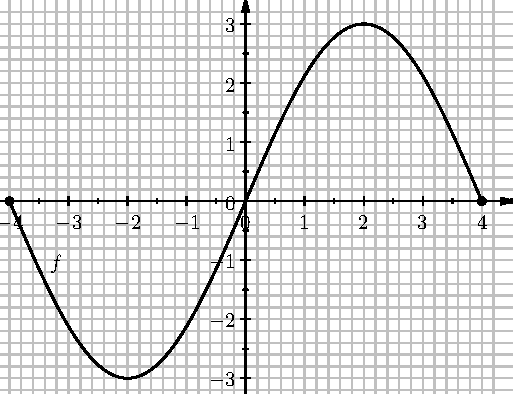
\includegraphics[scale=.7]{asys/funcion_3.pdf} 
  \end{minipage}\hfill
  \begin{minipage}{.45\textwidth}
    \item Dada la gráfica de la función $ f $
    \begin{enumerate}
      \item Estime $ f(0.5) $ usando una cifra decimal
      \item Estime $ f(3) $ aproximando a una cifra decimal
      \item Encuentre todos los números $ x $ en el dominio de $ f $ para los cuales $ f(x)=1 $
    \end{enumerate}
  \end{minipage}
  Para los ejercicios siguientes (6-11), dada la función $ f $
  \begin{itemize}
     \item Use geogebra para hacer la gráfica de $ f $
     \item Encuentre el dominio y el rango de $ f $ a partir de su gráfica
   \end{itemize}
   \begin{multicols}{2}
   \item $ f(x)=2(x+1) $  \item $ f(x)=-x^2 $
   \item $ f(x)=x^2+4 $ \item $ f(x)=-\sqrt{25-x^2} $
   \item $ \sqrt{x+2} $ \item $ \sqrt{16-x^2} $
   \end{multicols}
Para los ejercicios siguientes (12-17), haga la gŕafica de la función definida a trozos.
\begin{multicols}{2}
  \item $ f(x)=\left\{ \begin{array}{lcl}
    1 & \mbox{si} & x\leq1\\
    x+1 & \mbox{si} & x>1
  \end{array} \right. $
  \item $ f(x)=\left\{\begin{array}{lcl}
    1-x & \mbox{si} & x<-2\\
    5 & \mbox{si}& x\geq-2
  \end{array}\right. $
  \item $ f(x)=\left\{\begin{array}{lcl}
    2x+3 & \mbox{si} & x<-1\\
    3-x & \mbox{si} & x\geq-1
  \end{array} \right.$
  \item $ f(x)=\left\{\begin{array}{lcl}
    -1 & \mbox{si} & x<-1\\
    x & \mbox{si} & -1\leq x\leq1\\
    1 & \mbox{si} & x>1
  \end{array} \right.$
  \item $ f(x)=\left\{\begin{array}{lcl}
    1-x^2 & \mbox{si} & x\leq 2\\
    x & \mbox{si} & x>2
  \end{array} \right.$
  \item $ f(x)=\left\{\begin{array}{lcl}
    x^2 & \mbox{si} & |x|\leq1\\
    1 & \mbox{si} & |x|>1
  \end{array} \right.$
\end{multicols}
\end{enumerate}
\end{document}
